\documentclass[11pt]{article}
\usepackage[margin=1in]{geometry}
\usepackage{amsmath,amssymb}
\usepackage{array}
\usepackage{xcolor}
\usepackage{tikz}
\usepackage[colorlinks=true,linkcolor=blue,citecolor=blue,urlcolor=blue]{hyperref}
\usetikzlibrary{arrows.meta,positioning,calc}

\title{EMT Basics: A Practical Learning Guide for Power-System Electromagnetic Transients}
\author{Generated LaTeX Project}
\date{June 2026}

\newcommand{\pu}{\mathrm{pu}}
\newcommand{\dd}{\mathrm{d}}
\newcommand{\Vdc}{V_{\mathrm{dc}}}
\newcommand{\abc}{abc}
\newcommand{\dq}{dq}

\begin{document}
\maketitle

\begin{abstract}
This guide introduces the power-system, protection, electromagnetic transient, converter, control, simulation, and validation concepts needed to begin building and interpreting EMT studies. It emphasizes physical interpretation, common equations, small worked examples, and modeling practices that connect textbook theory with PSCAD-style studies. Classic references include Kundur for stability, Greenwood and Dommel for transients, Hingorani and Gyugyi for FACTS, and Yazdani and Iravani for voltage-source converters \cite{kundur1994,greenwood1991,dommel1969,hingorani2000,yazdani2010}.
\end{abstract}

\tableofcontents
\newpage

\section{Power System Fundamentals}
\begin{figure}[h]
\centering
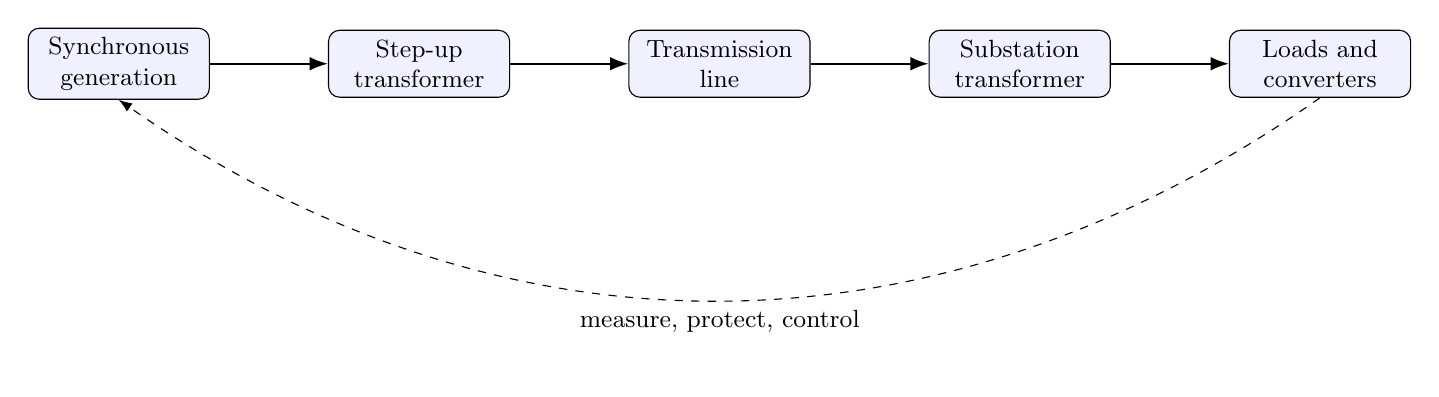
\begin{tikzpicture}[font=\small,>=Latex,node distance=1.5cm]
\tikzstyle{block}=[draw,rounded corners,minimum width=2.3cm,minimum height=0.85cm,align=center,fill=blue!6]
\node[block] (gen) {Synchronous\\generation};
\node[block,right=of gen] (xf1) {Step-up\\transformer};
\node[block,right=of xf1] (line) {Transmission\\line};
\node[block,right=of line] (xf2) {Substation\\transformer};
\node[block,right=of xf2] (load) {Loads and\\converters};
\draw[->,thick] (gen) -- (xf1);
\draw[->,thick] (xf1) -- (line);
\draw[->,thick] (line) -- (xf2);
\draw[->,thick] (xf2) -- (load);
\draw[->,dashed] (load.south) to[bend left=35] node[below]{measure, protect, control} (gen.south);
\end{tikzpicture}

\caption{A simplified power-system chain. EMT studies model each block at a level of detail appropriate to the frequency range of interest.}
\end{figure}

\subsection{Per Unit System}
The per-unit system normalizes voltage, current, impedance, and power to selected base values. For a three-phase system, choose $S_{\mathrm{base}}$ and line-to-line $V_{\mathrm{base}}$, then
\begin{equation}
I_{\mathrm{base}}=\frac{S_{\mathrm{base}}}{\sqrt{3}V_{\mathrm{base}}},\qquad
Z_{\mathrm{base}}=\frac{V_{\mathrm{base}}^2}{S_{\mathrm{base}}},\qquad
x_{\pu}=\frac{x_{\Omega}}{Z_{\mathrm{base}}}.
\end{equation}
\textbf{Example:} On a $100$ MVA, $230$ kV base, $Z_{\mathrm{base}}=(230\,\mathrm{kV})^2/100\,\mathrm{MVA}=529\,\Omega$. A $52.9\,\Omega$ reactance is therefore $0.10\,\pu$. Per-unit values are especially useful when transformers change voltage level because transformer turns ratios are absorbed by the base conversion.

\subsection{Three-Phase Systems}
Balanced three-phase systems use three sinusoidal phase quantities separated by $120^\circ$. Positive-sequence phasors rotate in the $a$-$b$-$c$ order, while negative sequence rotates oppositely and zero sequence has equal phase quantities. EMT programs often solve the instantaneous phase-domain network, while RMS tools often use positive-sequence phasors.

\subsection{Power Flow Concepts}
Power flow establishes pre-disturbance bus voltages and angles. For a line between buses 1 and 2 with series reactance $X$, the approximate active-power transfer is
\begin{equation}
P \approx \frac{|V_1||V_2|}{X}\sin(\delta_1-\delta_2).
\end{equation}
Reactive power is strongly affected by voltage magnitudes and shunt elements. In EMT initialization, a good power-flow solution prevents artificial transients at $t=0$.

\subsection{Transmission Line Modeling}
Short lines may be represented by lumped $R$, $L$, and $C$. Long lines require distributed parameters because voltage and current waves propagate with velocity $v\approx 1/\sqrt{LC}$ and characteristic impedance $Z_c=\sqrt{L/C}$. Frequency-dependent line models are important for lightning, switching surges, and cable resonance studies.

\subsection{Transformer Fundamentals}
Transformers transfer power through magnetic coupling, change voltage level, and provide phase shifts and grounding paths. EMT-relevant details include leakage reactance, winding resistance, saturation, inrush, residual flux, and zero-sequence behavior. A transformer specified as $x=0.12\,\pu$ on its own MVA base can be moved to a study base using $x_{\mathrm{new}}=x_{\mathrm{old}}(S_{\mathrm{new}}/S_{\mathrm{old}})(V_{\mathrm{old}}/V_{\mathrm{new}})^2$.

\section{Faults and Protection}
\begin{figure}[h]
\centering
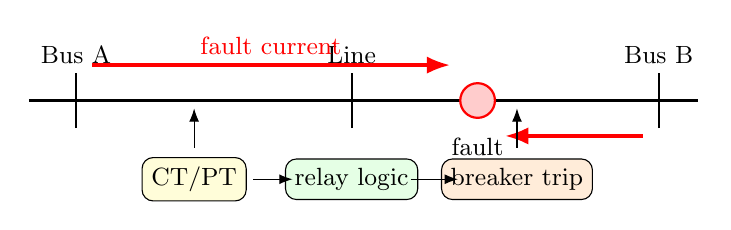
\begin{tikzpicture}[font=\small,>=Latex]
\draw[thick] (0,0) -- (8.5,0);
\foreach \x/\lab in {0.6/Bus A,4.1/Line,8.0/Bus B}{\draw[thick] (\x,-0.35)--(\x,0.35);\node[above] at (\x,0.35){\lab};}
\draw[fill=red!20,draw=red,thick] (5.7,0) circle (0.22);
\node[below=0.35cm] at (5.7,0) {fault};
\draw[->,very thick,red] (0.8,0.45) -- node[above]{fault current} (5.35,0.45);
\draw[->,very thick,red] (7.8,-0.45) -- (6.05,-0.45);
\node[draw,rounded corners,fill=yellow!15] at (2.1,-1.0) {CT/PT};
\node[draw,rounded corners,fill=green!10] at (4.1,-1.0) {relay logic};
\node[draw,rounded corners,fill=orange!15] at (6.2,-1.0) {breaker trip};
\draw[->] (2.1,-0.6)--(2.1,-0.1);
\draw[->] (2.85,-1.0)--(3.35,-1.0);
\draw[->] (4.85,-1.0)--(5.45,-1.0);
\draw[->] (6.2,-0.6)--(6.2,-0.1);
\end{tikzpicture}

\caption{Protection converts CT/PT measurements into a relay decision and breaker trip.}
\end{figure}

\subsection{Fault Analysis}
Fault analysis estimates currents and voltages during abnormal network conditions. A three-phase bolted fault is usually dominated by positive-sequence Thevenin impedance, $I_f=V_{\mathrm{prefault}}/(Z_1+Z_f)$. Single-line-to-ground faults use positive-, negative-, and zero-sequence networks in series. EMT simulations add dc offsets, saturation, arcing, and switching instants.

\subsection{Protection Basics}
Protection systems detect abnormal conditions, decide whether to trip, and isolate only the required equipment. Common elements include overcurrent, distance, differential, under/over-voltage, under/over-frequency, and directional functions. Selectivity, speed, sensitivity, reliability, and security are the main design tradeoffs.

\subsection{Breaker Operations}
Breakers interrupt current after relay and mechanical delays. EMT models should represent pole scatter, prestrike, restrike, current chopping, and transient recovery voltage when these effects matter. Standards in the IEEE C37 family provide breaker rating and testing guidance \cite{ieeec37}.

\subsection{CT/PT Behavior}
Current transformers and potential transformers scale primary quantities for relays and meters. CT saturation can distort fault-current waveforms and delay or misoperate protection. Coupling capacitor voltage transformers may produce subsidence transients that influence distance relay memory polarization.

\section{Electromagnetic Transients (EMT)}
\begin{figure}[h]
\centering
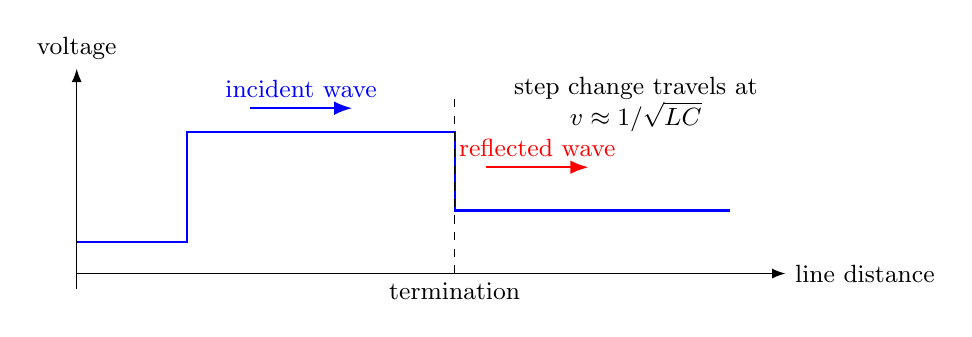
\begin{tikzpicture}[font=\small,>=Latex]
\draw[->] (0,0) -- (9,0) node[right]{line distance};
\draw[->] (0,-0.2) -- (0,2.6) node[above]{voltage};
\draw[thick,blue] (0,0.4) -- (1.4,0.4) -- (1.4,1.8) -- (4.8,1.8) -- (4.8,0.8) -- (8.3,0.8);
\draw[->,blue,thick] (2.2,2.1) -- node[above]{incident wave} (3.5,2.1);
\draw[->,red,thick] (5.2,1.35) -- node[above]{reflected wave} (6.5,1.35);
\draw[dashed] (4.8,0) -- (4.8,2.3);
\node[below] at (4.8,0){termination};
\node[align=center] at (7.1,2.15){step change travels at\\$v\approx 1/\sqrt{LC}$};
\end{tikzpicture}

\caption{A traveling voltage step and reflected wave on a distributed line.}
\end{figure}

\subsection{Time-Domain Analysis}
EMT tools solve differential and algebraic equations directly in time, commonly with trapezoidal integration as described by Dommel \cite{dommel1969}. A simple inductor update relates terminal voltage and current by $v=L\,\dd i/\dd t$. Time-domain analysis captures switching instants, nonlinear controls, saturation, and unbalanced conditions without assuming sinusoidal steady state.

\subsection{Switching Transients}
Switching energizes capacitors, transformers, lines, and reactors at a specific point on wave. The resulting transient depends on trapped charge, residual flux, network damping, and breaker pole timing. Controlled switching reduces overvoltages by closing at favorable voltage or flux conditions.

\subsection{Traveling Waves}
A surge on a line reflects and transmits whenever it reaches an impedance discontinuity. The voltage reflection coefficient is
\begin{equation}
\Gamma_v=\frac{Z_T-Z_c}{Z_T+Z_c},
\end{equation}
where $Z_T$ is the terminating impedance. Open circuits give $\Gamma_v\approx 1$ and short circuits give $\Gamma_v\approx -1$.

\subsection{Harmonics and Resonance}
Harmonics are integer multiples of the fundamental frequency produced by saturation, converters, and nonlinear loads. Resonance occurs when inductive and capacitive reactances cancel, magnifying voltages or currents. A simple series resonance frequency is $f_0=1/(2\pi\sqrt{LC})$.

\subsection{Ferroresonance}
Ferroresonance is a nonlinear resonance involving transformer saturation and capacitance. It can produce sustained overvoltages, irregular waveforms, and subharmonics. EMT simulation is preferred because the phenomenon is strongly nonlinear and depends on switching sequence and initial flux.

\section{Power Electronics}
\begin{figure}[h]
\centering
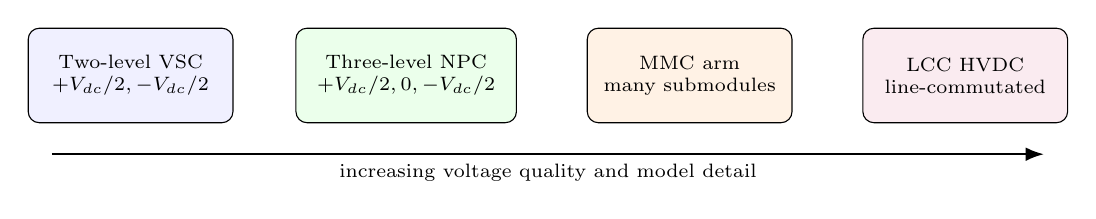
\begin{tikzpicture}[font=\scriptsize,>=Latex]
\node[draw,rounded corners,align=center,fill=blue!6,minimum width=2.6cm,minimum height=1.2cm] at (0,0) {Two-level VSC\\$+V_{dc}/2, -V_{dc}/2$};
\node[draw,rounded corners,align=center,fill=green!8,minimum width=2.8cm,minimum height=1.2cm] at (3.5,0) {Three-level NPC\\$+V_{dc}/2,0,-V_{dc}/2$};
\node[draw,rounded corners,align=center,fill=orange!10,minimum width=2.6cm,minimum height=1.2cm] at (7.1,0) {MMC arm\\many submodules};
\node[draw,rounded corners,align=center,fill=purple!8,minimum width=2.6cm,minimum height=1.2cm] at (10.6,0) {LCC HVDC\\line-commutated};
\draw[->,thick] (-1.0,-1.0)--node[below]{increasing voltage quality and model detail}(11.6,-1.0);
\end{tikzpicture}

\caption{Common converter families encountered in EMT studies.}
\end{figure}

\subsection{Converter Topologies}
Converter topology determines controllability, harmonic spectrum, losses, and required model detail. EMT models may represent ideal switches, averaged valves, or detailed semiconductor behavior depending on the study bandwidth.

\subsubsection{Two-Level VSC}
A two-level voltage-source converter switches each phase terminal between the positive and negative dc rails. It is simple and common in motor drives and smaller grid converters. Its phase voltage has high switching harmonics, so filters and PWM design are important.

\subsubsection{Three-Level NPC}
A neutral-point-clamped converter adds a midpoint level, reducing voltage steps and harmonics. Neutral-point voltage balancing is a key control task. NPC converters are useful when device voltage limits make two-level designs unattractive.

\subsubsection{MMC}
A modular multilevel converter uses many submodules per arm to synthesize a stepped waveform. MMC models include arm inductors, circulating current control, capacitor-voltage balancing, and insertion indices. Detailed MMC EMT models can be computationally heavy, so equivalent or averaged models are often used for system studies.

\subsubsection{LCC HVDC}
Line-commutated converters use thyristors and rely on the ac system voltage for commutation. They are robust for bulk power transfer but consume reactive power and are vulnerable to commutation failure in weak ac systems. Harmonic filters and reactive compensation are essential parts of LCC stations.

\subsection{PWM Techniques}
Pulse-width modulation maps a voltage reference into switch commands. Sinusoidal PWM is intuitive, space-vector PWM improves dc-bus utilization, and selective harmonic elimination targets specific harmonics. In EMT studies, the switching frequency should be resolved by the time step unless an averaged model is intentionally used.

\subsection{DC-Link Dynamics}
The dc-link capacitor balances converter ac and dc power. Neglecting losses, $C_{dc}\Vdc\,\dd \Vdc/\dd t=P_{dc}-P_{ac}$. Weak dc capacitance or aggressive controls can couple ac disturbances into dc-voltage oscillations.

\section{Inverter and Converter Controls}
\begin{figure}[h]
\centering
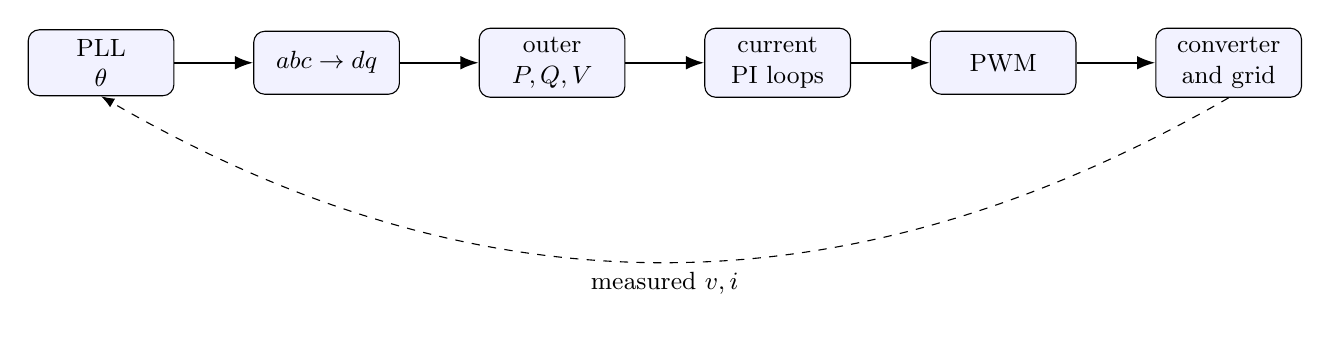
\begin{tikzpicture}[font=\small,>=Latex,node distance=1.0cm]
\tikzstyle{blk}=[draw,rounded corners,minimum width=1.85cm,minimum height=0.8cm,align=center,fill=blue!5]
\node[blk] (pll) {PLL\\$\theta$};
\node[blk,right=of pll] (abc) {$abc\to dq$};
\node[blk,right=of abc] (outer) {outer\\$P,Q,V$};
\node[blk,right=of outer] (inner) {current\\PI loops};
\node[blk,right=of inner] (pwm) {PWM};
\node[blk,right=of pwm] (plant) {converter\\and grid};
\draw[->,thick] (pll)--(abc);
\draw[->,thick] (abc)--(outer);
\draw[->,thick] (outer)--(inner);
\draw[->,thick] (inner)--(pwm);
\draw[->,thick] (pwm)--(plant);
\draw[->,dashed] (plant.south) to[bend left=30] node[below]{measured $v,i$} (pll.south);
\end{tikzpicture}

\caption{Typical grid-following converter control structure. Grid-forming controls replace the PLL-dependent reference with an internally generated voltage angle.}
\end{figure}

\subsection{dq Transformation}
The Park transform maps three-phase variables into a rotating reference frame. In a frame aligned with voltage, $v_q\approx 0$, active current $i_d$ primarily controls active power, and quadrature current $i_q$ primarily controls reactive power. Sign conventions must be checked carefully across tools.

\subsection{PLL (Phase Locked Loop)}
A PLL estimates grid angle and frequency from measured voltage. A synchronous-reference-frame PLL regulates $v_q$ to zero using a PI controller. In weak grids, PLL bandwidth can interact with grid impedance and converter current loops.

\subsection{Current Control Loops}
Current loops regulate converter currents and protect semiconductor limits. In the $dq$ frame, decoupling terms such as $\omega L i_q$ and $-\omega L i_d$ compensate cross-coupling. Bandwidth is typically set well below the switching frequency but faster than outer power or voltage loops.

\subsection{Voltage Control Loops}
Voltage loops regulate ac terminal voltage, filter capacitor voltage, or dc-link voltage. Their outputs often become current references. Excessive voltage-loop gain can create oscillations when grid strength is low.

\subsection{Outer and Inner Loop Controls}
Outer loops convert slow objectives such as active power, reactive power, ac voltage, or dc voltage into inner-loop references. Inner loops track current or voltage quickly. Time-scale separation is a useful design principle: inner loops should settle before outer loops demand large changes.

\subsection{Grid-Following Inverters}
Grid-following inverters inject controlled current synchronized to an external voltage using a PLL. They behave like current sources over their control bandwidth. They need a sufficiently strong voltage reference and may become unstable in very weak grids.

\subsection{Grid-Forming Inverters}
Grid-forming inverters establish voltage magnitude and frequency behind an impedance or virtual oscillator. They can energize islands and share load without an external phase reference. EMT models should include current limiting because limiting changes the apparent voltage-source behavior during faults.

\subsection{Droop Control}
Droop control emulates synchronous-machine sharing: frequency decreases as active power increases, and voltage decreases as reactive power increases. A common law is $\omega=\omega_0-m_p(P-P_0)$. Droop improves decentralized sharing but introduces steady-state deviations unless secondary control restores nominal values.

\subsection{Virtual Inertia}
Virtual inertia uses converter controls and stored energy to mimic the inertial response of rotating machines. A simplified swing-like equation is $M\dot{\omega}=P_m-P_e-D(\omega-\omega_0)$. Implementation must account for converter current limits and dc energy availability.

\section{Weak Grid and Stability Concepts}
\begin{figure}[h]
\centering
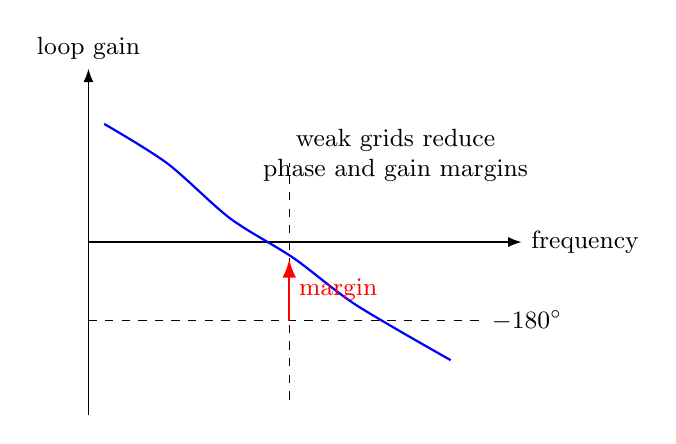
\begin{tikzpicture}[font=\small,>=Latex]
\draw[->] (0,0)--(5.5,0) node[right]{frequency};
\draw[->] (0,-2.2)--(0,2.2) node[above]{loop gain};
\draw[thick,blue] plot[smooth] coordinates{(0.2,1.5)(1.0,1.0)(1.8,0.3)(2.6,-0.2)(3.4,-0.8)(4.6,-1.5)};
\draw[dashed] (0,-1)--(5,-1) node[right]{$-180^\circ$};
\draw[dashed] (2.55,-2.0)--(2.55,1.0);
\node[align=center] at (3.9,1.1){weak grids reduce\\phase and gain margins};
\draw[->,red,thick] (2.55,-1) -- (2.55,-0.22);
\node[right,red] at (2.55,-0.6){margin};
\end{tikzpicture}

\caption{Weak grids reduce stability margins for converter controls and PLLs.}
\end{figure}

\subsection{Short Circuit Ratio (SCR)}
SCR measures grid strength at a point of interconnection: $\mathrm{SCR}=S_{sc}/P_{rated}$. Low SCR means grid voltage changes significantly for converter current injection. Very low SCR systems require careful tuning, grid-forming behavior, or additional compensation.

\subsection{Impedance-Based Stability}
Impedance-based analysis compares converter output impedance with grid impedance. Stability problems can appear when the ratio $Z_{grid}/Z_{converter}$ encircles the critical point in a Nyquist plot. EMT frequency scans and perturbation methods are common ways to obtain impedance models.

\subsection{Oscillatory Interactions}
Oscillations can arise from converter controls, series compensation, machine torsional modes, or weak-grid resonances. Important descriptors are frequency, damping ratio, participation, and triggering event. EMT waveforms reveal whether the oscillation is sinusoidal, saturating, or control-limited.

\subsection{Control Interactions}
Multiple controllers may regulate the same variable at similar bandwidths, producing adverse interactions. Examples include plant voltage controllers fighting inverter reactive-current controls, or PLLs interacting through a weak network. Coordination usually requires bandwidth separation and consistent droop or voltage priorities.

\subsection{Sub-Synchronous Oscillations}
Sub-synchronous oscillations occur below the fundamental frequency. Series-compensated lines can interact with turbine-generator shafts, while converter controls can introduce sub-synchronous control interactions. Damping controls and careful screening are required for renewable and HVDC interconnections.

\section{Control Systems}
\subsection{Transfer Functions}
Transfer functions relate Laplace-domain input and output under zero initial conditions, $G(s)=Y(s)/U(s)$. They are useful for small-signal analysis of linearized converter and machine controls. A first-order lag $G(s)=1/(1+sT)$ has a time constant $T$ and bandwidth near $1/T$.

\subsection{PI Controllers}
A PI controller has $G_c(s)=K_p+K_i/s$. The proportional term improves speed, while the integral term removes steady-state error. Anti-windup is necessary when actuators saturate, such as converter current or modulation limits.

\subsection{State-Space Modeling}
State-space models use $\dot{x}=Ax+Bu$ and $y=Cx+Du$. Eigenvalues of $A$ describe natural modes and damping. State-space form is convenient for multi-input multi-output controls and linearization around an operating point.

\subsection{Poles and Zeros}
Poles are roots of the denominator and define natural response. Zeros are roots of the numerator and shape input-output behavior. Right-half-plane poles indicate instability, and right-half-plane zeros impose bandwidth limits.

\subsection{Bode Plots}
Bode plots show magnitude and phase versus frequency. They help identify resonance peaks, crossover frequency, and phase lag. In converter controls, Bode plots are used to tune current loops, PLLs, and impedance-shaping controllers.

\subsection{Stability Margins}
Gain margin and phase margin quantify distance from instability in loop-gain analysis. A larger phase margin generally improves damping but may reduce speed. Weak-grid operation often lowers phase margin by adding plant delay and impedance coupling.

\subsection{Dynamic Response and Damping}
Dynamic response is judged by rise time, overshoot, settling time, and damping ratio. For a second-order mode, a damping ratio below about $5\%$ can be concerning in power-system studies. EMT simulation verifies whether nonlinear limits preserve the linearized damping expectation.

\section{Synchronous Machine Dynamics}
\subsection{Rotor Angle Dynamics}
Rotor angle dynamics follow the swing equation, $2H\dot{\omega}=P_m-P_e-D(\omega-1)$ in per unit. A disturbance accelerates or decelerates the rotor depending on the power imbalance. Transient stability studies examine whether machines remain in synchronism.

\subsection{Excitation Systems}
Excitation systems regulate generator field voltage and therefore terminal voltage and reactive power. Automatic voltage regulators improve voltage support but can interact with power-system stabilizers and limiters. EMT models may need saturation, ceiling voltage, and limiter details.

\subsection{Governors}
Governors regulate mechanical power and frequency response. Droop allows multiple units to share load changes. Governor dynamics are usually slower than EMT switching transients but are relevant for long-duration frequency and black-start studies.

\subsection{Transient and Subtransient Reactances}
Machine reactances change with time after a disturbance. Subtransient reactance $X''$ dominates the first cycles of fault current, transient reactance $X'$ follows, and synchronous reactance $X_d$ describes steady state. Protection and breaker duties often depend on the early subtransient current.

\subsection{Machine Inertia}
Inertia stores kinetic energy and slows frequency changes. The inertia constant $H$ is the stored kinetic energy at rated speed divided by machine MVA. Systems with high inverter penetration may have lower physical inertia and need fast frequency response or grid-forming controls.

\section{Renewable Energy Integration}
\subsection{Solar PV Plant Modeling}
PV plant models include irradiance-dependent dc sources, dc-link capacitors, inverter controls, collector systems, and plant-level controllers. EMT detail is needed for fault ride through, weak-grid stability, and control interactions. Averaged inverter models are often sufficient for slower plant control studies.

\subsection{Wind Turbine Modeling}
Wind models may represent type-3 doubly-fed induction generators or type-4 full-converter turbines. Important details include pitch control, torque control, converter current limits, crowbar behavior, and turbine transformer saturation. Mechanical shaft modes can matter for sub-synchronous studies.

\subsection{Plant-Level Controls}
Plant controllers coordinate many inverters to meet point-of-interconnection active-power, reactive-power, voltage, and frequency requirements. Communication delays and measurement filters influence stability. EMT studies should include realistic plant-control bandwidths rather than ideal instantaneous commands.

\subsection{Reactive Power Support}
Renewable plants provide reactive current through inverter controls, capacitor banks, STATCOMs, or SVCs. During faults, grid codes often prioritize reactive current to support voltage. The available reactive power is constrained by current rating and active-power output.

\subsection{Fault Ride Through (FRT)}
FRT requires resources to remain connected during specified voltage or frequency disturbances. Controls must manage current limits, dc-link energy, and PLL recovery. EMT simulation verifies whether protection, controls, and hardware limits coordinate through the event.

\subsection{LVRT/HVRT Requirements}
Low-voltage and high-voltage ride-through curves specify voltage-versus-time regions in which a plant must stay connected. IEEE 1547 gives interconnection requirements for distributed energy resources \cite{ieee1547}. Transmission-level grid codes may add reactive-current injection and recovery-rate requirements.

\section{Numerical Simulation Concepts}
\begin{figure}[h]
\centering
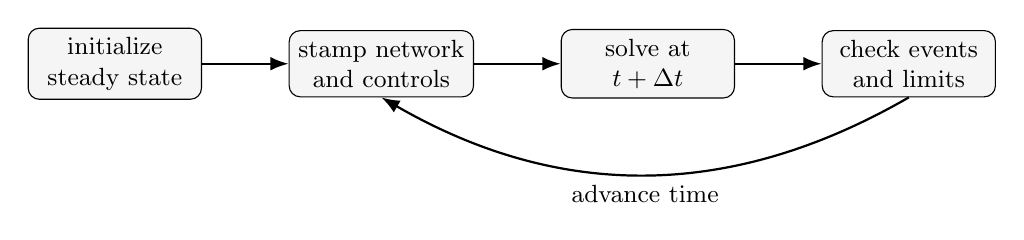
\begin{tikzpicture}[font=\small,>=Latex,node distance=1.1cm]
\tikzstyle{simstep}=[draw,rounded corners,align=center,minimum width=2.2cm,minimum height=0.8cm,fill=gray!8]
\node[simstep] (init) {initialize\\steady state};
\node[simstep,right=of init] (stamp) {stamp network\\and controls};
\node[simstep,right=of stamp] (solve) {solve at\\$t+\Delta t$};
\node[simstep,right=of solve] (check) {check events\\and limits};
\draw[->,thick] (init)--(stamp);
\draw[->,thick] (stamp)--(solve);
\draw[->,thick] (solve)--(check);
\draw[->,thick] (check.south) to[bend left=30] node[below]{advance time} (stamp.south);
\end{tikzpicture}

\caption{Basic EMT time-step workflow. Events such as breaker actions can force matrix refactorization or interpolation.}
\end{figure}

\subsection{EMT Solvers}
EMT solvers discretize network components into companion models and solve nodal equations at each time step. The trapezoidal method is accurate and widely used but can produce numerical oscillations after discontinuities. Damping or interpolation may be used when switching events occur.

\subsection{Time-Step Selection}
The time step must resolve the fastest modeled phenomenon. A $50\,\mu$s step can resolve fundamental-frequency electromechanical behavior and many controls, while detailed power-electronics switching may require $1$--$5\,\mu$s or smaller. Too large a step hides peaks and may destabilize controls.

\subsection{Numerical Stability}
Numerical stability depends on integration method, model stiffness, switching discontinuities, and control delays. Algebraic loops and ideal voltage-source conflicts are common causes of failure. Adding physically meaningful impedance or using proper interface models improves conditioning.

\subsection{Convergence Issues}
Nonlinear elements such as surge arresters, saturation, and power-electronic limits can cause convergence problems. Good initial conditions, realistic limits, and gradual energization help. If a case fails only at a switching instant, inspect event timing and discontinuities.

\subsection{Initialization Methods}
Initialization aligns EMT states with the desired steady-state operating point. Methods include power-flow import, phasor initialization, manual state setting, and pre-running to steady state. Poor initialization produces artificial inrush, dc offsets, or control transients.

\section{PSCAD-Specific Skills}
\subsection{PSCAD Master Library}
The PSCAD master library provides standard components for sources, lines, transformers, machines, controls, and measurements \cite{pscad}. Use library components first unless a custom model is required. Library documentation states assumptions and parameter units.

\subsection{Transmission Line Components}
PSCAD line components include Bergeron, frequency-dependent phase-domain, and cable models. Select the model based on line length, frequency range, and unbalance. Validate conductor geometry, transposition, grounding, and modal fitting.

\subsection{Transformer Components}
Transformer components represent leakage, winding connection, tap changers, magnetizing branches, and saturation. Include residual flux when studying energization. Check zero-sequence paths for grounded-wye, delta, and autotransformer connections.

\subsection{Breaker Modeling}
Breaker models can be ideal switches or detailed devices with timing, resistance, prestrike, and restrike. Use three independent poles when pole scatter affects transients. Confirm that opening/closing commands align with relay outputs and simulation event times.

\subsection{Machine Modeling}
Machine models require inertia, reactances, time constants, saturation, excitation, and governor data. Initialize machines to the desired P/Q output. For fault-current studies, verify subtransient parameters and grounding.

\subsection{Control Block Modeling}
Control block diagrams should match the implemented sampling, delays, limiters, and sign conventions. Use named signals and hierarchical pages for readability. Compare control outputs against hand calculations for simple test cases.

\subsection{Data Visualization}
Effective visualization includes RMS trends, instantaneous waveforms, spectra, and event markers. Plot per-unit and engineering units consistently. Zoom around switching instants to inspect peaks, not just long-window envelopes.

\subsection{Signal Processing in PSCAD}
Signal processing blocks include filters, RMS meters, Fourier analysis, zero-crossing detection, and sequence extraction. Filter delay matters when signals drive protection or controls. Sampling and window length determine harmonic resolution.

\subsection{Debugging PSCAD Models}
Debug by simplifying the model, checking initialization, forcing known inputs, and comparing with analytical results. Inspect units, base conversions, sign conventions, and limiter states. Save small benchmark cases that reproduce each issue.

\section{Model Validation and Testing}
\begin{figure}[h]
\centering
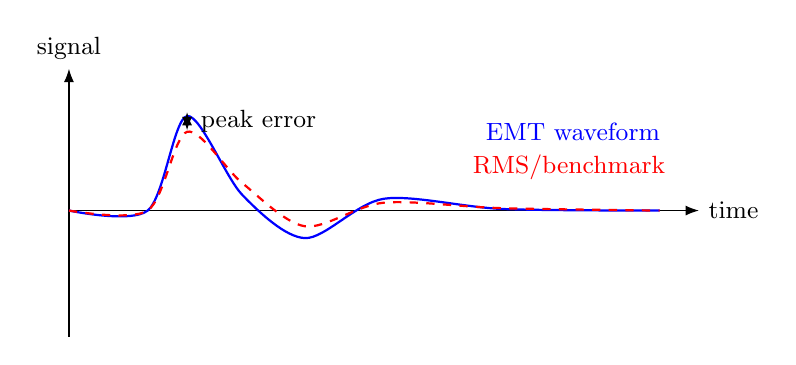
\begin{tikzpicture}[font=\small,>=Latex]
\draw[->] (0,0)--(8,0) node[right]{time};
\draw[->] (0,-1.6)--(0,1.8) node[above]{signal};
\draw[thick,blue] plot[smooth] coordinates{(0,0)(1,0)(1.5,1.2)(2.2,0.2)(3.0,-0.35)(4.0,0.15)(5.5,0.02)(7.5,0)};
\draw[thick,red,dashed] plot[smooth] coordinates{(0,0)(1,0)(1.5,1.0)(2.2,0.35)(3.0,-0.2)(4.0,0.1)(5.5,0.03)(7.5,0)};
\node[blue] at (6.4,1.0){EMT waveform};
\node[red] at (6.35,0.55){RMS/benchmark};
\draw[<->] (1.5,1.25)--(1.5,1.02);
\node[right] at (1.55,1.14){peak error};
\end{tikzpicture}

\caption{Waveform validation compares timing, peak, damping, and steady-state values against a benchmark.}
\end{figure}

\subsection{RMS vs EMT Comparison}
RMS and EMT tools should agree for balanced, fundamental-frequency behavior away from switching events. Differences are expected during unbalance, fast control action, saturation, and harmonics. Use the same power-flow initialization and equipment ratings before comparing.

\subsection{Waveform Validation}
Waveform validation checks peak value, phase, frequency, damping, settling time, and steady-state error. Align event times and use identical filtering before calculating errors. Always inspect both instantaneous and RMS quantities.

\subsection{Benchmark Testing}
Benchmark tests compare a model against a trusted analytical result, manufacturer data, field record, or published case. A transformer energization case, a line energization case, and a converter step-response case are useful starting benchmarks. Keep benchmarks small and repeatable.

\subsection{Sensitivity Studies}
Sensitivity studies vary uncertain parameters such as grid strength, control gains, transformer residual flux, line length, or fault impedance. They reveal whether conclusions depend on one fragile assumption. Report the parameter range and the response metric.

\subsection{Scenario Analysis}
Scenario analysis combines operating points, contingencies, protection actions, and control modes. Examples include high renewable output at low load, weak-grid faults, HVDC blocking, and black-start energization. Scenario matrices help ensure that a study covers credible extremes.

\section{HVDC and FACTS}
\subsection{VSC HVDC}
VSC HVDC uses self-commutated converters to control active and reactive power independently. It is well suited for offshore wind, weak grids, and black-start support. EMT models should include dc-cable dynamics, converter controls, and ac filters.

\subsection{LCC HVDC}
LCC HVDC is efficient for high-power long-distance transfer but needs strong ac systems for commutation. Commutation failure, reactive power demand, and harmonic filters are central study topics. Fault recovery depends on firing-angle controls and ac voltage support.

\subsection{STATCOM}
A STATCOM is a shunt VSC that injects reactive current to regulate voltage. It can provide fast dynamic support at low voltage better than mechanically switched capacitors. Current limits and control priorities should be represented in EMT studies.

\subsection{SVC}
A static var compensator uses thyristor-controlled reactors and switched capacitors. It provides shunt reactive compensation but generates harmonics and has voltage-dependent output. Its control bandwidth is generally lower than a STATCOM.

\subsection{Series Compensation}
Series capacitors reduce effective line reactance and increase power transfer capability. They can also introduce sub-synchronous resonance risk with turbine-generator shafts. Protection includes spark gaps, metal-oxide varistors, and bypass breakers.

\subsection{FACTS Controller Interactions}
Multiple FACTS devices may interact through voltage controls, damping controls, and network modes. Coordination studies should include realistic measurement filters, communication delays, and limiters. Hingorani and Gyugyi provide a broad introduction to FACTS technologies \cite{hingorani2000}.

\section{Industry and Grid Standards}
\subsection{NERC Standards}
NERC standards define reliability obligations for planning, operations, protection, and disturbance performance in North America. Studies often support compliance evidence, model quality, and event analysis. Always identify the applicable standard, region, and facility category.

\subsection{WECC Requirements}
WECC requirements and guidelines emphasize model validation, renewable plant representation, and disturbance performance for the Western Interconnection. WECC-style renewable models are common in RMS studies, while EMT models are used for weak-grid and control-interaction screening.

\subsection{ERCOT Interconnection Studies}
ERCOT interconnection studies evaluate voltage ride-through, reactive support, weak-grid stability, and system strength for resources connecting in Texas. EMT studies are often required for inverter-based resources in weak areas or near other power-electronic equipment.

\subsection{IEEE Standards}
IEEE standards cover interconnection, protection, breakers, transformers, measurement, and power quality. IEEE 1547 is especially important for DER interconnection \cite{ieee1547}. IEEE guides should be used with local grid-code requirements and utility practices.

\subsection{Grid Code Compliance}
Grid-code compliance links model studies to required plant behavior: ride-through, reactive current, frequency response, voltage regulation, harmonics, and power quality. The model should include the same protection and controls used in the field. Study reports should trace each requirement to an explicit scenario and pass/fail criterion.

\section{Mathematical Foundations}
\subsection{Complex Numbers}
Complex numbers represent sinusoidal phasors as magnitude and angle. Multiplication by $j$ rotates a phasor by $90^\circ$, and impedance is $Z=R+jX$. EMT waveforms are real time-domain signals, but phasors remain useful for initialization and interpretation.

\subsection{Differential Equations}
Inductors, capacitors, machines, and controllers are governed by differential equations. EMT simulation converts these equations into time-step updates. Analytical solutions for first- and second-order systems provide useful checks on simulated responses.

\subsection{Laplace Transforms}
Laplace transforms convert differential equations into algebraic equations in $s$. They support transfer-function modeling, block-diagram reduction, and stability analysis. Initial conditions must be handled carefully when comparing Laplace solutions to EMT simulations.

\subsection{Fourier Analysis}
Fourier analysis decomposes waveforms into frequency components. It is used for harmonic studies, resonance identification, and filter design. Window length, sampling rate, and leakage affect the accuracy of spectral estimates.

\subsection{Matrix Methods}
Power-system network equations use matrices such as the nodal admittance matrix $Y_{bus}$. State-space models use matrices for dynamic systems. Sparse matrix methods allow EMT programs to solve large networks efficiently at every time step.

\section{Advanced Topics}
\subsection{Real-Time Simulation}
Real-time simulation solves EMT equations fast enough to keep pace with wall-clock time. Fixed time steps and deterministic execution are required. Model detail must fit within the processor or FPGA time budget.

\subsection{Hardware-in-the-Loop (HIL)}
HIL connects real controllers, relays, or power hardware to a real-time simulator. It tests actual firmware and interfaces before field deployment. Signal scaling, latency, and amplifier limits must be included in the test plan.

\subsection{EMT-RMS Hybrid Simulation}
Hybrid simulation links detailed EMT areas with broader RMS networks. It is useful when a local converter-rich region needs EMT detail but the rest of the grid can remain phasor based. Interface errors and frequency-content assumptions must be validated.

\subsection{Wide-Area Oscillations}
Wide-area oscillations involve groups of generators or inverter plants swinging against each other over large distances. Monitoring uses synchrophasors, modal analysis, and damping estimates. Controllers such as power-system stabilizers, HVDC modulation, or grid-forming controls can add damping.

\subsection{Black Start Studies}
Black start studies evaluate energizing a system from de-energized conditions. EMT issues include transformer inrush, motor starting, temporary overvoltage, protection coordination, and converter grid-forming capability. Sequential restoration plans should be tested against equipment limits.

\subsection{Protection Coordination}
Protection coordination ensures primary and backup devices operate in the correct order. Time-current curves, distance zones, differential boundaries, and communication-assisted schemes must be checked. EMT studies are valuable when CT saturation, dc offset, inverter fault current, or breaker transients affect relay inputs.

\section*{Learning Path}
\addcontentsline{toc}{section}{Learning Path}
A practical learning sequence is: (1) master per-unit and three-phase fundamentals; (2) simulate simple RL, LC, line, transformer, and fault cases; (3) add protection and breaker timing; (4) study converter average and switching models; (5) tune PLL, current, voltage, and outer loops; (6) screen weak-grid interactions; and (7) validate against benchmarks and standards. Keep a library of small cases with known answers so that every new model can be tested before it is placed in a large network.

\bibliographystyle{plain}
\bibliography{references}
\end{document}
